\documentclass[a4paper,oneside]{book}

%% Language and font encodings
\usepackage[frenchb]{babel}

\usepackage[utf8]{inputenc}
\usepackage[T1]{fontenc}

\usepackage{verbatim}
\usepackage{enumitem}

% creation de la commande circled, mot entoure d'un cercle
\newcommand*\circled[1]{\tikz[baseline=(char.base)]{% <---- BEWARE
            \node[shape=circle,draw,inner sep=2pt, color=pumpkin] (char) {#1};}}

% quotes package
\usepackage[autostyle, maxlevel = 2]{csquotes}

% bibliography package            
\usepackage[backend = biber, style = numeric]{biblatex}   
\addbibresource{references.bib}            

% glossary package
\usepackage[toc]{glossaries}

% loading glossary file
\loadglsentries{Glossaire/glossaire.tex} 
\makeglossaries

% package for references and links 
\usepackage{caption}

% package for insertion of pdf pages
\usepackage{pdfpages}

% package to change behavior of floats numbering
\usepackage{chngcntr}
\counterwithout{figure}{chapter}

% pour les images
\usepackage{graphicx}
\usepackage{caption} 
\usepackage{float} 
\usepackage{wrapfig}

%% pour les tableaux
\usepackage{array}
\usepackage{tabularx}
\usepackage{multirow}
\usepackage{slashbox}
\usepackage{colortbl}
\usepackage{framed}
\usepackage{adjustbox}

% pour les maths
\usepackage{amsmath}
\usepackage{amsfonts}
\usepackage{amssymb}
\usepackage{mathrsfs}  
\usepackage{pifont}
\newcommand{\cmark}{\ding{51}}
\newcommand{\xmark}{\ding{55}}

%% package for landscape page view
\usepackage{lscape}

%% pour dessiner des graphiques et des schemas
\usepackage{tikz}
\usepackage{tkz-graph}
\usetikzlibrary{calc, decorations.pathreplacing}

% Pgfplots
\usepackage{pgfplotstable}
\usepackage{pgfplots}
\usetikzlibrary{pgfplots.groupplots}
\pgfplotsset{compat=1.12}

% définitions des couleurs
\usepackage{color}
  \definecolor{grey}{rgb}{0.4,0.4,0.4}
  \definecolor{blue}{rgb}{0.2,0.3,0.6}
  \definecolor{teal}{rgb}{0.1,0.4,0.4}
  \definecolor{green}{rgb}{0.1,0.7,0.2}
  \definecolor{red}{rgb}{0.8,0.1,0.2}
  \definecolor{pumpkin}{rgb}{0.9, 0.3, 0}

%% Pour l'intégration de code SQL
\usepackage{listings} 
\usepackage{listingsutf8}
\lstloadlanguages{JAVA, SQL}
\lstset{ % affichage du code par défaut
    inputencoding=utf8/latin1,
    basicstyle=\footnotesize\sf,
    morecomment=[s]{/*}{*/},
    morecomment=[l]{//}, 
    keywordstyle=\sffamily\bfseries\color{teal},
    commentstyle=\itshape\color{grey},
    stringstyle=\rmfamily\color{pumpkin},
    tabsize=2, frame=single, breaklines=true,
    showspaces=false, showstringspaces=false,extendedchars=true, 
    numbers=left, numberstyle=\tiny,
    extendedchars=true,
    literate={\$}{{{\$}}}1 {é}{{\'e}}1,    
}

%% definition de style pour une ligne entiere d'un tableau
\newcolumntype{+}{>{\global\let\currentrowstyle\relax}}
\newcolumntype{^}{>{\currentrowstyle}}
\newcommand{\rowstyle}[1]{\gdef\currentrowstyle{#1}%
#1\ignorespaces
}

%% Sets page size and margins
\usepackage[a4paper,top=2cm,bottom=2cm,left=2cm,right=2cm,marginparwidth=1.75cm]{geometry}

%% Pour ecrire des algorithmes
\usepackage[vlined,ruled,linesnumbered]{algorithm2e}

%% Useful packages
\usepackage{amsmath}
\usepackage{amssymb}
\usepackage{amsthm}
\theoremstyle{definition}
\newtheorem{example}{Example}

\usepackage[colorinlistoftodos]{todonotes}
\usepackage[colorlinks=true, allcolors=blue]{hyperref}
\usepackage{nameref}

\usepackage{titlesec}
\titleformat{\chapter}[display]{\flushleft\Huge\itshape}{\quad}{0.5em}{}[]
\titleformat{\paragraph}[runin]{\normalfont\normalsize\bfseries}{}{0pt}{}

% leaves out chapter numbers in section numbering
\renewcommand*\thesection{\arabic{section}}

% command defining new chapter type, to be used whith roman page numbering
\newcommand\romanchapter[1]{
  \chapter*{#1}
  \markboth{\MakeUppercase{#1}}{}
  \addcontentsline{toc}{chapter}{#1}
}

\usepackage{fancyhdr}
\setlength{\headheight}{15.2pt}
\pagestyle{fancy}

\begin{document}

\begin{titlepage}
\begin{center}
\begin{sffamily}

{\large
Faculté de Sciences de Montpellier \\[.5cm]
Master 2 AIGLE\\2017 -- 2018\\[2cm]
}


% Title
\rule{\textwidth}{1.6pt}\vspace*{-\baselineskip}\vspace*{2pt} 
\rule{\textwidth}{0.4pt}\\[\baselineskip]
{\LARGE
Notation symbolique de flux de contrôle musicaux et multimédias\\[0.7\baselineskip]

\includegraphics[width=0.2\textwidth]{Paratextes/i/logo.jpg}
\\[0.5\baselineskip]
Rapport bibiliographique
}\\[0.2\baselineskip] 
\rule{\textwidth}{0.4pt}\vspace*{-\baselineskip}\vspace{3.2pt}
\rule{\textwidth}{1.6pt}\\[\baselineskip]
\vspace*{2\baselineskip}

% Author and supervisor
\noindent
\begin{center}
     \large
    \emph{\textbf{Étudiant:}}\\
    Vincent Iampietro \\
    \smallskip
    \large
    \emph{\textbf{Encadrant:}}\\
    Jean Bresson\\
    \emph{\textbf{Co-encadrant:}}\\
    Rama Gottfried
\end{center}%



\end{sffamily}
\end{center}
\end{titlepage}

%%%%% PAGE DE GARDE %%%%%
\pagenumbering{Roman}

\setcounter{tocdepth}{1} % profondeur du sommaire, 1 pour sections uniquement

%%%%% SOMMAIRE %%%%%%
\tableofcontents

%%%%% INTRODUCTION %%%%%
\chapter{Introduction}
	La notation musicale peut être distinguée en deux approches : un approche prescriptive et une approche descriptive \cite{battier2015}.
La notation prescriptive a pour but de décrire \og comment la musique doit sonner \fg.
Dans cette optique, la partition fait office de référence ou du moins de repère pour l'interprétation d'une pièce. 
La notation descriptive tente de retranscrire \og comment la musique a sonné \fg.
Ainsi, à des fins d'analyse, une pièce peut être caractérisée et fixée sur une partition.
Cependant, la partition reste l'outil privilégié du compositeur pour la communication de sa musique, et, au-delà de l'objet fini, constitue également un espace de travail.\\
Aussi, la préparation d'une pièce contemporaine par un ensemble musical se fait souvent en collaboration avec le compositeur. La partition constitue alors le support de la discussion et se voit même être modifiée pour les besoins de l'exécution de la pièce.\\
Comme le dit Carmine E. Cella, chercheur et compositeur à l'IRCAM, en parlant de l'écriture musicale : \og le créateur doit s'efforcer de trouver un compromis notationnel entre sa pensée et la réalisation pratique de sa pièce \fg. L'annexe \ref{sec:refletsDeLOmbre} donne deux exemples de partitions représentant la même partie de la pièce \textit{Reflets de l'ombre} (C. E. Cella, 2013), montrant l'adaptation de la notation à des fins d'exécution.
En définitive, une troisième approche de la notation musicale pourrait se profiler, celle d'une conception \textit{évolutive} de la partition.
\clearpage

\stepcounter{page}
\pagenumbering{arabic}

%%%%% CHAPITRE "DE LA NOTATION MUSICALE" %%%%%
\chapter{De la notation musicale}
\label{chap:deLaNotation}

	\todo{Ajouter une intro pour le chapitre}	
	
	\section{Un peu d'histoire}
	\label{sec:unPeuDHistoire}
	L'évolution perpétuelle de la notation musicale témoigne du caractère versatile de la pensée compositionnelle, qui est fonction de trois entités : le compositeur, l'interprète et le cadre socio-technologique d'une époque\cite{bosseur2005}.
A travers l'histoire, la présente partie veut suggérer au lecteur la difficulté de l'écriture musicale, et la nécessité de sa réinvention constante.
Pour plus de clarté, le choix a été fait de découper l'évolution de la notation musicale en périodes historiques. Aussi, le caractère continuel du développement de la Musique n'est pas entièrement respecté.   

\paragraph{Antiquité et Moyen-Age} Le premier exemple d'une notation musicale apparaît au IIIe siècle av. J-C en Grèce avec la notation \textit{boécienne}. A cette époque, les notes de la gamme sont représentées par des lettres de l'alphabet.
Cette représentation est conçue dans une acception théorique pure visant à modéliser la relation entre les sons musicaux et les matières scientifiques, notamment les mathématiques.

Au IXe siècle, plusieurs exemples de parchemins retranscrivant des chants liturgiques sont annotés par des symboles appelés \glspl{neume} (voir annexe \ref{sec:exempleTexteNeume} page~\pageref{sec:exempleTexteNeume}). 
Ces symboles ont pour de but de décrire approximativement les inflexions mélodiques de la voix. Par exemple, le neume "point" (\textit{punctum}) indique le chant d'une note isolée; le neume "virgule" (\textit{virga}), représenté par un accent aigu, indique le chant à un intervalle supérieur vis à vis d'un neume "point".
Déjà, la notation neumatique témoigne de la volonté de fixation des caractéristiques du son chanté par le symbole. Ici, la dimension fixée est la hauteur relative des sons entre eux.

Par la suite, la notation carrée (1175-1225, voir annexe \ref{sec:exempleNotationCarree} page~\pageref{sec:exempleNotationCarree}), suivie par la notation noire (1250-1450), factorisent la profusion symbolique des neumes et coïncident avec la volonté de noter les pièces polyphoniques qui font leurs apparitions entre le Xème et XIème siècle.
La \gls{polyphonie}\footnote{Combinaison de plusieurs voix ou parties mélodiques, dans une composition musicale.} cristallise l'intérêt des compositeurs pour les relations de durée entre les différentes voix; petit à petit une notation rythmique va voir le jour.

Entre le XIIIème et le XIVème siècle, la barre verticale représentant la mesure fait son apparition sur la portée. La mesure regroupe, en ce temps, les ensembles de notes selon le mode rythmique employé dans la pièce musicale.
Dans la continuité de cette période, les symboles de notes se multiplieront et mèneront à une fixation absolue des valeurs rythmiques (c'est à dire, à un symbole est associé une durée).

Au XIIIème siècle, une \gls{portee} stable (quatre barres pour la liturgie, cinq barres pour les autres chants) fait son apparition. Ainsi, la hauteur des notes devient fixée strictement, notamment par l'apposition de clés (clé de Fa, de Ut et de Sol\footnote{Il est a noté que l'apparition des noms des notes de la gamme date du XIème siècle environ. Les noms correspondent au premières lettres d'un hymne à Saint Jean-Baptiste :
\textbf{UT} queant laxis - \textbf{RE}sonare fibris - \textbf{MI}ragestorum - \textbf{FA}muli tuorum -  \textbf{SOL}ve pollueti - \textbf{LA}billi reatum - \textbf{S}ancte \textbf{I}ohannes}) au début de la partition.

La fin du XIVème siècle voit poindre "une phase de complication et d'intrications inégalées"\cite[43]{bosseur2005} en termes de notation musicale. Vient s'ajouter à la variété des symboles musicaux un système de couleur qui adjoint une sémantique rythmique supplémentaire aux pièces musicales.\\
Cette période correspond à l'âge d'or des moines-copistes, ce qui explique l'émulation notationnelle qui fait ressembler les partitions à de véritables œuvres graphiques, délaissant la compréhension des pièces par les interprètes. \\
Comme le fait remarquer Jean-Yves Bosseur, cette tendance se retrouvera au XXème siècle avec la diversité des notations apportée par la musique contemporaine. 
   
\paragraph{De la renaissance au romantisme} Au XVème siècle, l'invention de l'imprimerie conduit à la standardisation de l'écriture musicale. Les notes prennent peu à peu une forme arrondie du fait des techniques d'impression. Les fractions, indiquant la signature rythmique au sein des mesures, font également leurs apparitions. 

Malgré l'unification de la notation, une grande liberté d'interprétation est laissée aux musiciens exécutants. De la renaissance (du XVème au XVIème siècle) jusqu'à l'époque baroque (du XVIIème au milieu du XVIIIème siècle), les partitions deviennent très épurées (voir annexe \ref{sec:exempleMusiqueBaroque}); elles ne conservent que la structure basique des pièces. Le reste est laissé à la discrétion de l'interprète : une manière de rester lié avec la tradition orale héritée du Moyen-Age.

La fin du XVIIème siècle voit apparaître de nouveaux symboles fixant les effets d'ornementations mélodiques sur la portée. Une moindre place est accordée à la liberté de jeu de l'interprète, qui devient de plus en plus dépendant de la notation musicale.\\
Progressivement, le métier de compositeur s'affirme, et, la fin du XVIIIème siècle portant avec elle les idéaux de la révolution française, la singularité des œuvres musicales est de plus en plus fixée sur la partition, dans la proclamation du droit moral inhérent de l'auteur sur ses œuvres.\\
A l'ère du romantisme (XIXème siècle), la notation s'intéresse à fixer plus finement les caractéristiques du son et de l'interprétation. Des nouveaux symboles apparaissent pour transcrire le doigté des instruments, la dynamique du son (\textit{nuances}) ou le mode d'accentuation des notes (voir annexe \ref{sec:exempleNotationInterpretation}).

\paragraph{Le XXème siècle} Par la suite, deux tendances se dessinent qui cohabiteront tout au long du XXème siècle. 

La première est à l'augmentation de la partition traditionnelle, dans le but de traduire avec précision les nouvelles formes musicales qui apparaissent à cette époque.\\
Par exemple, le compositeur Schoenberg introduit le \textit{dodécaphonisme} pour rompre avec la \gls{tonalite}\footnote{Une tonalité se définit comme une gamme de sept notes, désignée par sa tonique et son mode (majeur ou mineur). Par exemple, tonalité de Do majeur (Do = tonique, majeur = mode).}. Il imagine alors un nouveau type de portée qui mettrait à niveau égal chacun des douze sons de la gamme chromatique. Il voit dans l'augmentation de l'espace de représentation une manière de transcrire plus fidèlement sa musique.\\
Dans une autre démarche, le compositeur et ethnomusicologue Béla Bart\'{o}k essaye de retranscrire les musiques folkloriques à tradition orale entendues au cours de ses voyages d'investigation.
Cependant, il se heurte à la difficulté de noter avec un système limité des pratiques musicales particulières :

\begin{displayquote}[{\cite[94]{bosseur2005}}]
\og Dans les mélodies populaires, il y a beaucoup de sons étrangers, certains glissements de voix, des sons dont la hauteur ne peut être exactement précisée.\fg 
\end{displayquote}

L'impuissance de Belà Bart\'{o}k à pouvoir noter certaines musiques lui fera dire que "la vraie partition se trouve sur les pistes du disque", résultat des enregistrements fait sur place.\\
Cette déclaration montre la limitation de la notation musicale, qui ne peut porter à elle seule toute la diversité et la complexité de la musique de cette époque.

Partant de ce constat, une autre tendance notationnelle apparaît, laissant plus de place à l'interprétation et à l'improvisation. \\
En effet, les compositeurs de la deuxième moitié du XXème siècle (Stockhausen, Cage, Brown…) \og estiment volontiers que la notation, loin de s'efforcer de "conserver" les caractéristiques d'une œuvre -- tâche dont peuvent aujourd'hui se charger les moyens de reproduction mécanique avec une minutie inégalée par tout autre système de transcription -- devrait plutôt constituer un catalyseur pour le jeu musical. \fg (\cite[115]{bosseur2005}).\\
Ainsi, les partitions prennent un envers de plus en plus graphique, déconstruisant la notation "traditionnelle", et laissant le rôle de témoin d'une œuvre aux moyens technologiques.\\
La partition devient même une œuvre graphique en soi, et donne lieu à des expositions. La première prend place en 1959 à Donaueschingen, où sont présentées les partitions du compositeur Anestis Logothetis (voir annexe \ref{sec:exempleAnestisLogothetis}).

Durant les années 50, la musique électroacoustique naît grâce aux outils électroniques de synthèse audio\-phonique. 
La composition se fait alors à même la matière sonore, sans intervention préalable d'une transcription symbolique des pièces.
Ainsi, la notation des œuvres électroacoustiques intervient souvent, dans une optique d'analyse, après leur production (\textit{représentation descriptive}, voir section \ref{subsec:butDeLaNotation}).\\
De même, la notation de telles pièces s'écartent du symbolisme de la notation traditionnelle; une relation continue au temps est préférée au système métrique\footnote{Système basé sur la décomposition du temps selon une nombre de pulsations par minute.}.

\bigskip

L'Histoire nous apprend que noter la Musique est une démarche en fluctuation constante. L'acte notationnel est fonction avant tout de la place que prennent le compositeur, l'interprète et même l'auditeur dans la tendance musicale liée à une époque.
De même, la notation se standardise aux siècles où la portée constitue le médium d'échange par excellence et le support de l'interprétation : à la renaissance après l'invention de l'imprimerie, jusqu'à l'époque romantique.
En revanche, la notation se diversifie aux époques où la mémorisation des œuvres musicales est déléguée à d'autres médiums : au Moyen-Âge à la grande tradition orale, ou au XXème siècle avec les technologies d'enregistrement du son.   

Aujourd'hui, la diversité des approches et modes de production de la Musique rend quasi impossible l'unification sa notation.
Au contraire, la direction inverse serait à privilégier :
\begin{displayquote}[{\cite[133]{bosseur2005}}]
\og Noter, ce n'est plus alors nécessairement indiquer une hauteur de son, un rythme…, noter, c'est aussi inventer une écriture.\fg 
\end{displayquote} 


	
	\section{Noter la musique contemporaine}
	\label{sec:noterLaMusiqueContemporaine}
	Même si la pluralité des approches musicales amène à l'éclatement d'une pratique notationnelle unique, la partition n'en reste pas moins \og un moyen pour le compositeur de penser sa musique, la décrire et la communiquer grâce à un système de représentation symbolique \fg \cite{bresson2008}.
En effet, le projet \textit{symbolist}, qui constitue le cadre du présent stage de recherche, a été impulsé par Jean Bresson et Rama Gottfried, dans l'optique d'offrir aux compositeurs de musique \textit{contemporaine} un outil informatique pour la spécification de leur propre notation.
Par conséquent, cette partie s'intéresse à la définition de la musique contemporaine et expose les problématiques liées à son écriture.

\subsection{Définition}
Selon Wikipédia :

\begin{displayquote}
\og La musique contemporaine représente les différents courants de musique savante apparus après la fin de la Seconde Guerre mondiale \fg.
\end{displayquote}

Etant donné la multitude de mouvements musicaux jonchant la période des années 50 à aujourd'hui,
une définition plus restrictive est proposée au lecteur : 

\begin{displayquote}
La musique contemporaine fait référence à toute pratique compositionnelle et artistique, qui, par l'entremise de moyens et supports divers empruntés au domaine audiovisuel (instruments de musique, ordinateurs, installation physique…), se constitue en vecteur d'une expérience sonore, voir multisensorielle (visuelle, tactile…). Cette musique est également caractérisée par sa pleine intégration des outils électroniques et numériques dans le processus créatif.
\end{displayquote}

Comme illustration de la musique contemporaine, un fragment de la partition de la pièce \textit{Fluoresce} (R. Gottfried, 2012) est présentée en figure \ref{fig:schemaInstallationFluoresce}.

\begin{figure}[H]
	\centering
	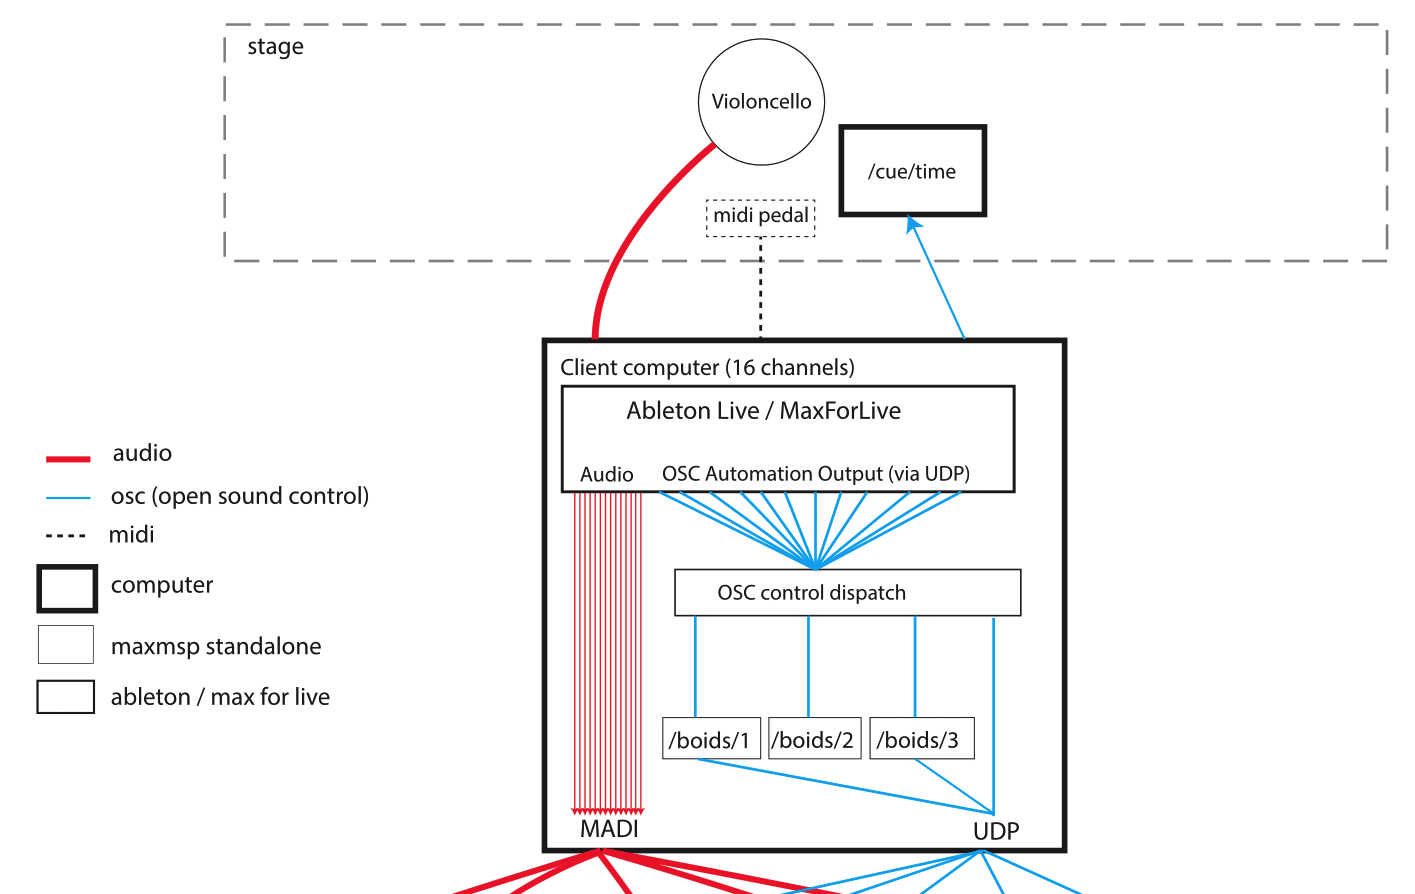
\includegraphics[keepaspectratio=true, width=\textwidth]{Notation/i/schemaInstallationFluoresce.png}
	\caption[Schéma de branchement pour la pièce \textit{Fluoresce} par Rama Gottfried]{Schéma de branchement pour la pièce \textit{Fluoresce} par Rama Gottfried}
	\label{fig:schemaInstallationFluoresce}			
\end{figure}
\begin{center}
\small \it La figure \ref{fig:schemaInstallationFluoresce} présente le schéma de câblage des différents éléments qui vont servir à l'exécution de la pièce. La performance fait intervenir un joueur de violoncelle (\textit{Violoncello}); le son produit par le violoncelle est capté et envoyé à un ordinateur (\textit{Client computer}) sur lequel est lancé la station audionumérique\footnote{\og Une station audionumérique (acronyme DAW, de l'anglais digital audio workstation) désigne […] un ensemble d'outils électroniques, conçu pour enregistrer, éditer, manipuler, créer et lire des contenus audionumériques.\fg -- Wikipédia} \textit{Ableton Live} associé au plugin \textit{MaxForLive}\footnote{MaxForLive est un plugin permettant l'intégration du logiciel Max/MSP à la station audionumérique Ableton Live. Voir plus loin pour plus de détails sur Max/MSP.}. Ableton Live répartit le signal audio sur les systèmes WFS et HOA (\textit{Wave Field Synthesis} et \textit{High Order Ambisonics}\footnote{\textit{Wave Field Synthesis} et \textit{High Order Ambisonics} sont deux systèmes de diffusion de sons spatialisés basés sur l'utilisation d'un grand nombre d'enceintes.}) via la liaison MADI\footnote{MADI (Multichannel Audio Digital Interface) est une liaison audionumérique définissant un protocole capable d'embarquer 64 canaux audio simultanément}. Le plugin MaxForLive envoie des messages OSC\footnote{Open Sound Control. Protocole de communiaction entre ordinateurs, synthéthiseurs et autres appareils. \textbf{Voir le chapitre} pour plus de détails.} \texttt{/boids/1}, \texttt{/boids/2} et \texttt{/boids/3} (directives de déclenchement d'effets sonores), via UDP, aux systèmes WFS et HOA. Le schéma de branchement complet est consultable en annexe \ref{sec:schemaInstallationFluoresceComplet} page~\pageref{sec:schemaInstallationFluoresceComplet}. L'écoute et la description de la pièce \textit{Fluoresce} sont accessibles à l'url \url{http://www.ramagottfried.com/fluoresce.html}.
\end{center}

Cette pièce met bien en place des moyens audiovisuels (un violoncelle, des ordinateurs, et deux systèmes de diffusion sonore…) pour traduire une expérience musicale; ici l'expérience est purement sonore, il n'y a pas de dimension multisensorielle. La pièce \textit{Fluoresce} est un type de musique appelée "musique mixte", c'est à dire qui mélange instruments traditionnels et Informatique.

Sur le schéma, l'ordinateur sur scène envoie le message OSC \texttt{/cue/time} au \textit{Client computer}. Le message \texttt{/cue/time} transmet un référentiel temporel permettant la synchronisation entre le jeu du violoncelliste et le \textit{Client computer}. 
Dans le cas de musique mixte, la question de la synchronisation humain/machine et du suivi de partition est centrale (voir la section suivante). 
En effet, même si une pièce de musique contemporaine peut se détacher de toutes notions de métrique, de mélodie et d'harmonie, elle admet tout de même un ordonnancement temporel des éléments la composant.
D'ailleurs, sur les partitions du XXème siècle, Jean-Yves Bosseur indique que la notation agit comme le \og déclencheur d'une chaîne d'actions et de réactions sonores \fg (\cite[121]{bosseur2005}), illustrant bien l'impératif de temporisation et de synchronisation inhérent à la musique contemporaine.

Pour finir, la présence d'un schéma de branchement au sein de la partition de \textit{Fluoresce} démontre la nécessité d'augmentation de la portée traditionnelle, qui n'est pas capable de retransmettre à la fois le contenu et l'agencement d'une pièce musicale.

\subsection{But de la notation pour la musique contemporaine}
\label{subsec:butDeLaNotation}
La notation musicale peut être distinguée en deux approches : un approche prescriptive et une approche descriptive \cite{battier2015}.

La notation prescriptive a pour but de décrire \og comment la musique doit sonner \fg.
Dans cette optique, la partition fait office de référence ou du moins de repère pour l'interprétation d'une pièce. 

La notation descriptive tente de retranscrire \og comment la musique a sonné \fg.
Ainsi, à des fins d'analyse, une pièce peut être caractérisée et fixée sur une partition.

La musique contemporaine hérite de la musique électroacoustique son caractère expérimental. Ainsi, la composition d'une telle musique s'effectue souvent à même la matière sonore, sans l'entremise de la partition.\\
Aussi, quel est l'objectif de la notation pour la musique contemporaine?\\
De nombreuses pièces électroacoustiques n'ont été notées qu'après coup par les musiciens les produisant (exemple, les truc-muches…). Ainsi, dans le cas de la musique contemporaine une approche descriptive de la notation serait à envisager.

Cependant, la partition reste l'outil privilégié du compositeur pour la communication de sa musique, et, au-delà de l'objet fini, constitue également un espace de travail.\\
Aussi, la préparation d'une pièce contemporaine par un ensemble musical se fait souvent en collaboration avec le compositeur. La partition constitue alors le support de la discussion et se voit même être modifiée pour les besoins de l'exécution de la pièce.\\
Comme le dit Carmine E. Cella, chercheur et compositeur à l'IRCAM, en parlant de l'écriture musicale : \og le créateur doit s'efforcer de trouver un compromis notationnel entre sa pensée et la réalisation pratique de sa pièce \fg.\\
L'annexe \ref{sec:refletsDeLOmbre} donne deux exemples de partitions représentant la même partie de la pièce \textit{Reflets de l'ombre} (C. E. Cella, 2013), montrant l'adaptation de la notation à des fins d'exécution.

En définitive, une troisième approche de la notation musicale pourrait se profiler, celle d'une conception \textit{évolutive} de la partition.

\subsection{Problématiques liées à la notation de la musique contemporaine}
\label{subsec:pbmatiquesMusiqueContemporaine}	

%%%%% CHAPITRE "OUTILS INFORMATIQUES POUR LA NOTATION DE LA MUSIQUE"
\chapter{Outils informatiques pour la notation de la Musique}
\label{chap:outilsInfo}
\rhead{\textit{OUTILS INFORMATIQUES}} % change title right of the header

La présente partie dresse, d'en un premier temps, un état de l'art des logiciels et langages permettant de noter la Musique.
De même, elle tend a montré l'insuffisance de telles ressources pour ce qui est de noter la musique contemporaine.
Le chapitre se décline en trois parties : la section \ref{sec:outilsNotationSymbolique} présente les outils informatiques permettant d'écrire la Musique à l'aide de symboles, incluant ceux de la notation standard; la deuxième partie expose les moyens informatiques pour une notation morphologique de la Musique, c'est à dire, basée sur une représentation visuelle de l'onde sonore; la troisième partie s'intéresse aux outils évolués, ajoutant une dimension "interactive" à la portée, faisant d'eux de véritables environnements de création.   

	\section{Outils pour une notation musicale symbolique}
	\label{sec:outilsNotationSymbolique}
	\lhead{\textit{NOTATION SYMBOLIQUE}}
L'avantage d'une notation symbolique de la Musique réside dans sa capacité à être lue plus aisément par des humains. Bien sûr, pour interpréter une partition "symbolique", le lecteur a toujours besoin de connaître la sémantique des symboles qui lui sont présentés. Ainsi, la notation conventionnelle de la Musique ne sonnent qu'aux oreilles des praticiens du solfège.

Cependant, l'Informatique vient bouleverser le schéma traditionnel d'interaction entre la partition, l'interprète et l'auditeur \cite{gottfried2017}. L'ordinateur peut prendre la place de l'interprète et faire entendre la partition à l'auditeur; il peut lire les symboles d'une partition et produire le son (lecture d'un fichier audio, synthèse sonore…) associé à chaque symbole. \\
Par conséquent, loin de penser à un total remplacement des interprètes humains par des interprètes numériques, l'ordinateur se présente comme un outil d'apprentissage des symboles et de leur sémantique, en agissant comme un démonstrateur au service du compositeur.  

Au vue de ces nouvelles considérations, et prenant en compte les challenges soulevés par la musique contemporaine (voir chapitre \ref{chap:deLaNotation}, section \ref{subsec:pbmatiquesMusiqueContemporaine}), les outils présentés dans cette section seront évaluées en fonction des critères suivants :
Est-ce que le logiciel intègre la notation standard ? Est-ce que le logiciel permet la création de nouveaux symboles musicaux ? Permet-il d'associer une sémantique aux nouveaux symboles créés ?

\subsection{Outils de notation à base de compilateurs}
\label{subsec:notationABaseCompilateurs}
Un premier type de logiciels, proposant une notation symbolique de la Musique, permet de décrire textuellement une partition, puis de compiler le texte pour générer le résultat graphique.
De nombreux paramètres de mise en page de la partition sont gérés automatiquement à la compilation (espacement des notes, gestion des retours à la ligne…), ce qui permet au compositeur de se concentrer sur le contenu de son œuvre.

\paragraph{MusiXTeX} Le langage MusiXTeX, basé sur le processeur de texte \TeX, est un des outils permettant de générer une portée graphique à partir de texte. MusiXTeX a besoin de trois passes de compilation (1 passe \TeX, 1 passe \textit{musicflx}, et 1 passe \TeX) pour pouvoir calculer un espacement horizontal adéquat entre les notes et ensuite générer le document pdf.

MusiXTeX fournit les symboles de la notation standard, ainsi que des symboles musicaux moins répandus, accessibles dans ses nombreuses extensions (par exemple, l'extension \textit{musixgre} permet l'utilisation de la notation carrée, voir \hyperref[sec:unPeuDHistoire]{Un peu d'histoire}).\\
Pour représenter les notes, MusiXTeX utilise le système anglo-saxon (maintenant système international), dans lequel les sept premières lettres de l'alphabet $a, b, c, d, e, f, g$ correspondent respectivement aux notes la, si, do, ré, mi, fa, sol. Pareillement, les valeurs rythmiques de notes sont introduites par les balises \lstinline{\wh} (ronde, \textit{whole note}), \lstinline{\h} (blanche, \textit{half note} en anglais), \lstinline{\q} (noire, \textit{quarter note} en anglais)… 


MusiXTeX ne permet pas la création de nouveaux symboles pour la portée, et l'intégration de symboles écrits avec d'autre package \LaTeX, comme \textit{tikz}, est complexe voir impossible.
Aussi, le rendu final de la compilation est un fichier pdf, donc un format purement graphique. La partition produite n'est pas interprétable par ordinateur.

\paragraph{Lilypond} Lilypond est un autre générateur de portée, logiciel libre rattaché au projet \textit{GNU} \cite{lilypond2018}. Son système de notation est semblable à celui de MusiXTeX (il existe d'ailleurs un package Lilypond pour \LaTeX), avec plus de légèreté syntaxique, et une communauté d'utilisateurs et de développeurs bien plus active.
Le listing \ref{lst:lilypond} donne une idée de la définition d'une structure de portée en Lilypond.

\begin{lstlisting}[caption={Ecriture de partition avec Lilypond}, 
					label=lst:lilypond, captionpos=b, language=Java]
\score {
	<<
		// Création d'une nouvelle voix sur la portée
		\new Staff = "singer" <<
			...
		>>
		
		// Création d'une voix pour piano		
		\new PianoStaff = "piano" <<
			...
		>>
	>>
}
\end{lstlisting}

Lilypond fournit son propre compilateur (le binaire \textit{lilypond}) pour générer un fichier pdf en sortie. Un fichier MIDI\footnote{\og Le Musical Instrument Digital Interface ou MIDI est un protocole de communication et un format de fichier dédiés à la musique, et utilisés pour la communication entre instruments électroniques, contrôleurs, séquenceurs, et logiciels de musique.\fg -- Wikipédia} correspondant à la partition peut également être généré, en incluant la balise \lstinline|\midi{}| dans la balise \lstinline|\score{}|; la partition est donc interprétable par ordinateur.

L'utilisateur peut modifier à son aise les propriétés graphiques des éléments de la partition, et même créer de nouveaux symboles à l'aide de la balise \lstinline|\markup nomDuSymbole args|. Grâce à cette possibilité d'augmentation de la portée par de nouveaux symboles, il existe de nombreux exemples de pièces contemporaines notées avec Lilypond. Pour l'exemple, une pièce de Mike Solomon est visible en annexe \ref{sec:luckyWokSolomon}.

De plus, le compilateur Lilypond inclus le moteur \textit{Guile}, implémentation du langage \textit{Scheme}, qui permet l'intégration de scripts \textit{Scheme} à la syntaxe Lilypond. De fait, les capacités algorithmiques d'un langage de programmation générique sont mises au service de l'écriture de partition.

Cependant, et c'est la critique majeure qui peut être adressée aux systèmes à compilateur, la définition de nouveaux symboles graphiques reste complexe, et nécessite d'être rompu à la pratique des langages de programmation.
De même, lorsqu'un nouveau symbole est créé, Lilypond ne permet pas de lui associer une sémantique, qui lui permettrait, par exemple, d'être transcrit au format MIDI et interprété par l'ordinateur.

\paragraph{GUIDO} GUIDO, spécifié à l'origine par Holger H. Hoos et Keith Hamel, est un format pour la notation de la Musique \cite{hoos1998}. GUIDO permet uniquement d'utiliser la notation standard pour décrire la portée. Lors de sa création, le langage GUIDO n'était accompagné d'aucun compilateur permettant de générer un rendu graphique ou sonore à partir du texte. Par la suite, le GUIDO Engine a été développé par le SALIERI Group puis le GRAME (centre national de création musicale basé à Lyon), pour permettre la visualisation graphique de la portée à partir du format GUIDO. 

Même si le format GUIDO ne permet aucune intégration de nouveaux symboles, ni de convertir le texte en un format sonore, la concision de sa syntaxe et l'existence de SDKs pour le GuidoEngine en font un outil facilement intégrable dans un logiciel de notation musicale. Par exemple, l'environnement pour partition augmentée Inscore (voir section ), aussi développé par le GRAME, utilise le format GUIDO pour la partie notation standard de la Musique.    

\subsection{Outils de notation wysiwyg}
\label{subsec:outilsWysiwyg}

De nombreux outils de notation musicale wysiwyg (pour \textit{what you see is what you get}) existent dans le domaine libre et commercial. Parmi les plus populaires, \textit{Finale} (MakeMusic) et Sibelius (Avid) sont des logiciels propriétaires payants, et \textit{Musescore} et \textit{NoteAbility} font partie du monde libre.

Leur interface graphique présentent les mêmes caractéristiques : la portée fait office d'élément central, accompagnée d'une palette des symboles inscriptibles et d'un lecteur permettant de jouer la partition.
Les logiciels wysiwyg de notation inclus systématiquement un moteur d'interprétation MIDI pour le rendu audio de la pièce musicale.
La figure \ref{fig:sibeliusScreenshot} donne une vue du logiciel Sibelius présentant les éléments cités ci-dessus.

\begin{figure}[H]
	\centering
	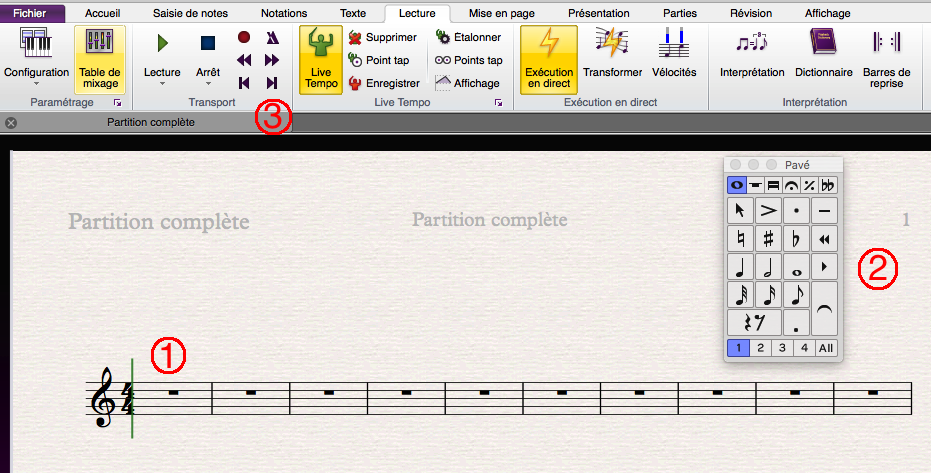
\includegraphics[keepaspectratio=true, width=0.8\textwidth]{OutilsInformatiques/i/sibeliusScreenshot.png}
	\caption{Capture d'écran du logiciel Sibelius}
	\label{fig:sibeliusScreenshot}
	\small \it
	En 1, la portée. En 2, la palette (appelé "pavé" dans Sibelius) des symboles de la notation standard.
	En 3, la barre de transport permettant la lecture et le jeu de la partition. 			
\end{figure}

L'interface graphique de tels logiciels facilite l'écriture de partitions par tous types d'utilisateurs-musiciens, là où les outils de notation à compilateur nécessitaient une connaissance de la programmation informatique.

Cependant, les logiciels actuels ne permettent que très difficilement de sortir des sentiers battus de la notation standard pour créer de nouveaux symboles et leur associer une sémantique. Les trois systèmes les plus répandus que sont \textit{Sibelius}, \textit{Finale} et \textit{Musescore} proposent la fonctionnalité d'insertion d'images pour ajouter de nouvelles entités musicales à une partition. En revanche, la palette ne peut pas être étendue par de nouveaux symboles, et la modification du graphisme des figures existantes ne fait pas partie du comportement naturel de ces programmes.

\paragraph{NoteAbility} Le logiciel \textit{NoteAbility} fait figure d'exception en ce qu'il offre à l'utilisateur une grande liberté dans la modification du graphisme de la portée et des symboles musicaux \cite{noteAbility2018}.
Il intègre même des outils d'édition graphique qui confère la possibilité de dessiner à même la portée, comme le montre la figure \ref{fig:exempleNoteAbility}.
Également, une sémantique particulière peut être associée à des symboles en leur adjoignant des messages, qui seront envoyés sur un port UDP particulier lors de la lecture. Ces messages peuvent être reçus par n'importe quel logiciel écoutant le port en question, et transcris en interprétation sonore.

\begin{figure}[H]
	\centering
	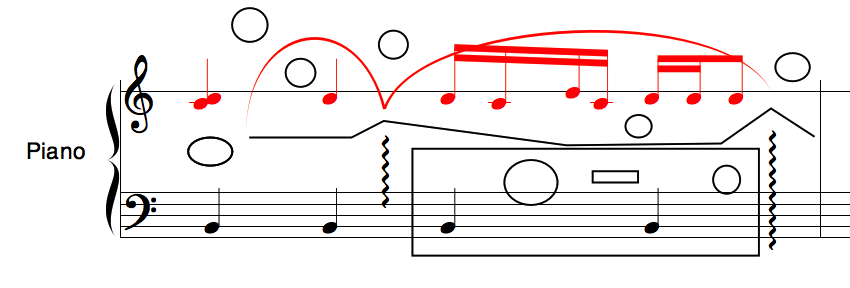
\includegraphics[keepaspectratio=true, width=0.8\textwidth]{OutilsInformatiques/i/exempleNoteAbility.png}
	\caption{Exemple de création graphique avec NoteAbility Pro}
	\label{fig:exempleNoteAbility}			
\end{figure}

Toutefois, \textit{NoteAbility} ne permet pas de sauvegarder les nouveaux symboles créés dans la palette des \textit{Music Images} (terme utilisé pour qualifier les symboles musicaux). Cette fonctionnalité est annoncée pour les versions à venir.

\paragraph{Iannix}
 
	
		
	
%%%%% CONCLUSION %%%%%
\chapter{Conclusion}
Comme peut en témoigner l'Histoire, la notation musicale n'est pas un processus monolithique. L'écriture de la musique est influencé par le contexte technologique propre à chaque époque. Aussi, la musique contemporaine, qui s'installe à partir des années 50, voit ses pratiques profondément impactées par l'usage de l'électronique et l'informatique. Aujourd'hui encore, l'apparition de nouvelles technologies (machine learning, réalité virtuelle, IoT\footnote{Internet of Things}…) pousse les compositeurs à réinventer leur relation avec la musique et la manière de la noter. Au-delà de la musique contemporaine, la composition multimédia, tirant profit de la profusion des supports technologiques de notre époque (vidéo, audio, capteurs, actionneurs…), cherche encore un système de notation qui lui serait adéquat. Au moment de la rédaction de cette étude, les technologies pour la création musicale sont trop récentes et trop nombreuses pour pouvoir proposer une pratique notationnelle unique. De fait, chaque compositeur a ses propres besoins en termes d'écriture, ce qui devrait pousser les outils informatiques à proposer plus de fonctionnalités permettant l'invention d'une notation par l'utilisateur.

Or, les logiciels actuels de notation musicale ne répondent qu'en partie à la prérogative d'extensibilité ou de renouveau des pratiques d'écriture de la musique, dans le but de s'accorder avec la création contemporaine. Une première catégorie des logiciels existants intègre bien la notation traditionnelle mais ne fournissent que peu de moyens pour l'étendre et l'adapter à l'écriture d'œuvres nouvelles. Une deuxième catégorie de logiciels approche la transcription musicale sous l'angle des pièces électroacoustiques et multimédias, en incorporant aux partitions une dimension interactive. Cependant, cette seconde catégorie de logiciels délaisse quelque peu l'expressivité symbolique au profit de la description temporelle des processus régissant les œuvres.

Dans ce contexte, le développement du logiciel \textit{symbolist} a été initié afin d'adresser le problème du manque d'outils permettant de transcrire symboliquement les œuvres contemporaines \cite{gottfried2018}.
\textit{symbolist} est un éditeur graphique libre où le compositeur peut créer à volonté tous types de symboles et les enregistrer dans une palette. Ce logiciel est destiné à être encapsulé dans les environnements \textit{OpenMusic} et \textit{Max}, et utilise le protocole OSC pour s'interfacer avec l'extérieur.
La poursuite du développement de \textit{symbolist} constitue le cadre du présent stage. Aussi, la génèse et les caractéristiques du logiciel seront explicitées dans le rapport final d'activités.
Dans la continuité de la période d'étude bibliographique, un recueil du besoin sera effectué auprès des compositeurs de musique contemporaine (de l'IRCAM et d'ailleurs), afin de déterminer précisément les attentes des utilisateurs potentiels de \textit{symbolist}.
De plus, une démarche d'analyse et de rétro-ingénierie sera mené sur le logiciel, étant donné son état avancé de développement.
Enfin, une étape d'organisation et de planification des méthodes de travail sera préalable à l'implémentation de nouvelles fonctionnalités.   
 

\stepcounter{page}
\pagenumbering{Roman}

%%%%% BIBLIOGRAPHIE %%%%%
\printbibliography
\addcontentsline{toc}{chapter}{Bibliographie}

%%%%% TABLE DES FIGURES %%%%%
\listoffigures
\addcontentsline{toc}{chapter}{Table des figures}

%%%%% GLOSSAIRE %%%%%
\printglossary[title={Glossaire}, toctitle={Glossaire}]

%%%%% ANNEXES %%%%%
\lhead{} % remove the left part of the header (section name)
\rhead{\textit{ANNEXES}} % set right header
\appendix
\romanchapter{Annexes}
% Pour faire une référence d'une annexe
% (Annexe \ref{sec:nomsection} page~\pageref{sec:nomsection})



\end{document}
